\section{Fundamentals of Machine Learning}
\subsection{Bridging Machine Learning and Artificial Intelligence}
In the rapidly evolving domain of computer science, Artificial Intelligence (AI) and Machine Learning (ML) exhibit a compelling interrelationship,
particularly promising in an era abundant with data. As the demand for intelligent applications escalates, it becomes imperative to distinguish
clearly between these two frequently conflated terms. As critically highlighted by Kühl et al.\cite{ai_and_ml_2020}, the terms AI and ML are often
used interchangeably both in scholarly literature and expert discussions, leading to considerable ambiguity.

Essentially, ML can be seen as a subset of AI, primarily focused on designing systems that autonomously learn from data and enhance their
performance over time without explicit reprogramming.In contrast, a widely acknowledged definition of AI, as provided by Russell and
Norvig\cite{russell_norvig_book}, positions AI as "the study of agents that receive percepts from the environment and perform actions."
On this basis, the authors classify AI systems into four types: Those that think like humans, think rationally, act like humans, and act
rationally.

Building on this classification, it provides a fundamental framework for understanding the diverse objectives and methodologies within AI research.
It emphasizes AI’s ability to perceive its environment through data acquisition and respond through actions, thereby linking it closely with fields
such as machine learning, robotics, natural language processing, and reasoning. This clear delineation not only helps in understanding AI's broad
applications but also illustrates the foundational role of ML within the broader AI landscape.
% \begin{figure}[!ht]
%     \centering
%     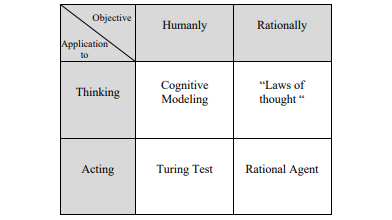
\includegraphics[width=0.7\textwidth]{./figures/ml/ai_streams.png} % Adjust the width to 50% of the text width
%     \caption{AI research streams based on Norvig.}
%     \label{fig:ml_taxonomy}
% \end{figure}

%%%%%%%%%%%%%%%%%%%%%%%%%%%%%%%%%%%%%%%%%%%%%%%%%%%%%%%%%%%%%%%%%%%%%%%%%%%%%%%%%%%%%%%%%%%%%%%%%%%%%%%%%%%%%%%%%%%%%%%%%%%%%%%%%%%%%%%%%%%%%%%%%%%%%%%%%%%%%%
\subsection{The Taxonomy Machine Learning Techniques}
Now that a clear distinction between the terms AI and ML is established, it is crucial to examine the nature of the diverse methodologies encompassed
by ML\@. The generalisability of published research on this issue remains a challenge. Over recent years, various studies have offered differing
classifications of ML methods, with the determining factor being the scope under which ML was investigated. Predominantly, existing literature has been
concentrated on the nature of the feedback mechanism applied, primarily categorizing ML algorithms into supervised, unsupervised and semi-supervised
~\cite{edge_computing_ml_2023, ml_big_data_2019} with some studies also incorporating reinforcement learning into their analysis
~\cite{survey_ml_big_data_2016, sarker_ml_algorithms_2021}.

This research, however, adopts a more holistic approach, aspiring to grasp the whole spectrum of ML applications. Instead of focusing solely on the
nature of the learning feedback, this classification also considers the objectives of the learning tasks and the timing of data availability. This
broader taxonomy, initially introduced by Zhou et al.\cite{zhou_ml_big_data_challenges_2017}, encapsulates all the critical elements that influence
the design and deployment of ML algorithms. The suggested taxonomy is the one shown below in \cref{fig:ml_taxonomy}.

\begin{figure}[!ht]
    \centering
    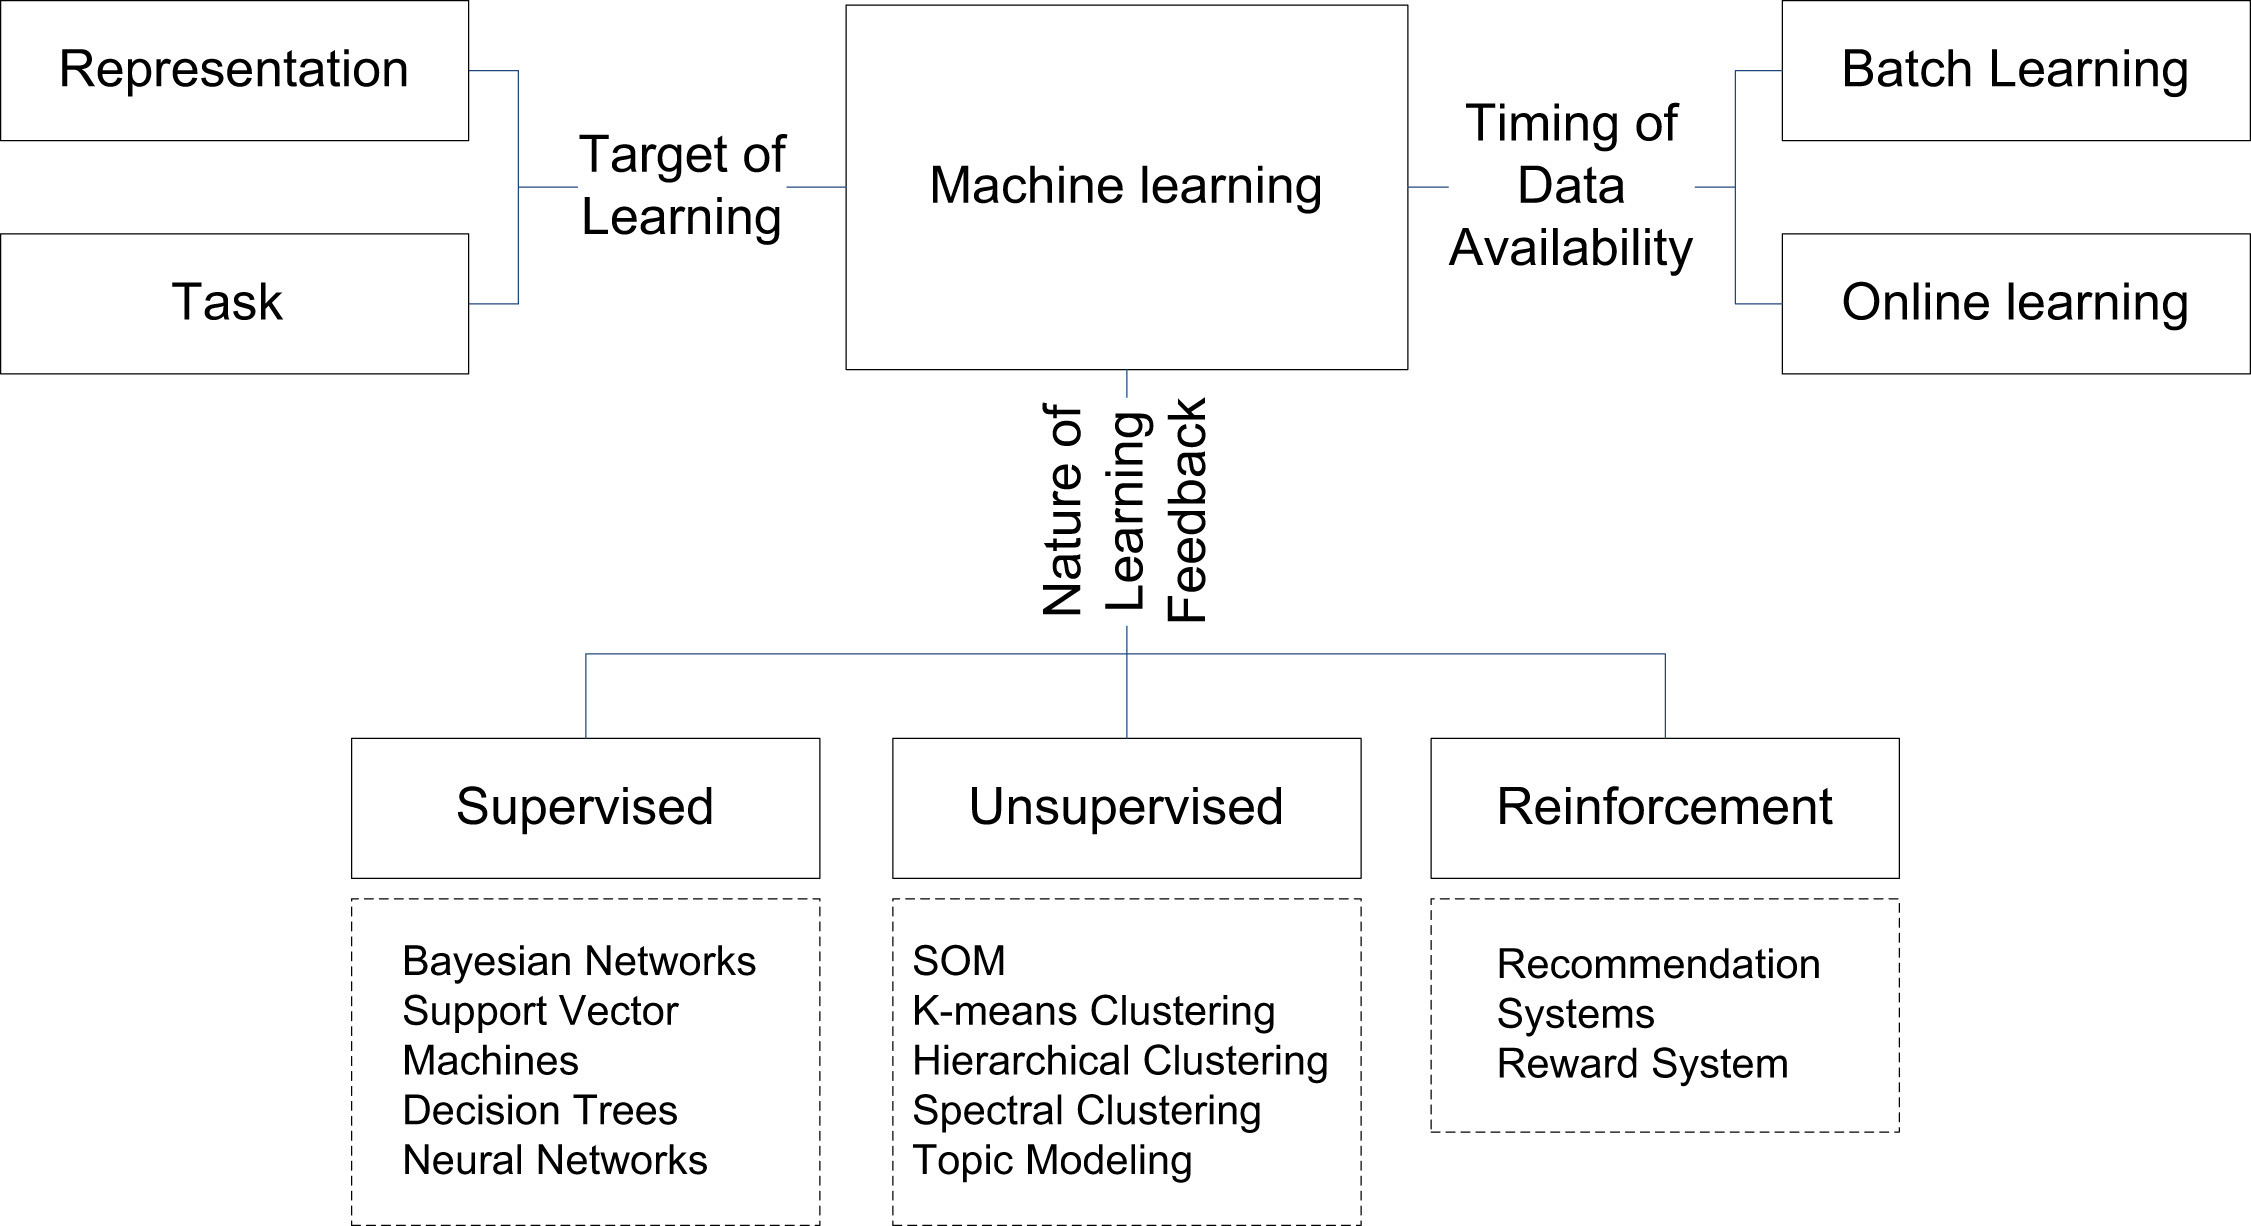
\includegraphics[width=.95\textwidth, keepaspectratio]{./figures/ml/ml_structure.jpg}
    \caption{Multi-dimensional taxonomy of Machine Learning\cite{zhou_ml_big_data_challenges_2017}.}
    \label{fig:ml_taxonomy}
\end{figure}

\begin{itemize}
    \item \textbf{Nature of Learning Feedback:} Based on this dimension of the taxonomy applied to Machine Learning, three principal system categories and one secnondary system
          emerge: supervised, unsupervised, and reinforcement learning systems and semi-supervised (secondary). In supervised learning, sample input-output pairs are presented to the
          system, which in turn attempts to infer a function able to map inputs to corresponding outputs. In practical terms, supervised ML techniques strive
          to construct a predictive model by applying algorithms to a set of known data points to extrapolate insights to an unseen dataset\cite{sarker_ml_algorithms_2021,hastie_statistical_learning_2017}.

          Unsupervised learning, in contrast, can be identified as a more data-driven approach, where datasets devoid of labels are analyzed. This means that while
          the structure of the data is apparent; no explicit guidance is provided as to the expected outcome and the aim is to uncover inherent patterns within
          the data without predefined answers.

          Likewise, reinforcement learning is not provided with input-output pairs, thus resembling unsupervised learning.
          Yet it requires a form of feedback—namely rewards or penalties linked to the actions taken. This environment-driven feedback mechanism guides the
          learning process towards optimal decision-making in an effort to minimize loss or maximize reward, depending on the environment's setup\cite{spyropoulos_lectures_2023}.
          The distinct applications of these techniques are demonstrated by Qiu et al.\cite{survey_ml_big_data_2016}, who assert that supervised and unsupervised
          learning primarily concentrates on data analysis, whereas reinforcement learning is better suited for decision-making tasks.

          Additionally, semi-supervised learning which sits at the intersection of supervised and unsupervised learning, entails learning from a limited set of
          labeled data complemented by a larger pool of unlabeled data. The aim of this learning method is similar to supervised learning, yet the
          knowledge is gathered both from annotated and unannotated data. Some of the key algorithmic examples of each category are demonstrated in the following \cref{table:feedback_taxonomy};

          \begin{table}[h!]
              \centering
              \begin{tabularx}{\textwidth}{>{\hsize=0.7\hsize\arraybackslash}X >{\hsize=1.8\hsize\arraybackslash}X >{\hsize=0.5\hsize\arraybackslash}X}
                  \toprule
                  \rowcolor{lightgray}
                  \textbf{Learning type} & \textbf{Model building}                                & \textbf{Examples}          \\
                  \midrule
                  Supervised             & Algorithms learn from labeled data (task-driven)       & Classification, regression \\
                  Unsupervised           & Algorithms learn from unlabeled data (data-driven)     & Clustering, associations   \\
                  Semi-supervised        & Models built using combined data (labeled + unlabeled) & Classification, clustering \\
                  Reinforcement          & Models based on reward or penalty (environment-driven) & Classification, control    \\
                  \bottomrule
              \end{tabularx}
              \caption{Learning types based on feedback along with key examples of each field}
              \label{table:feedback_taxonomy}
          \end{table}

    \item \textbf{Target of Learning:} Machine learning can be segmented into representational and task learning based on the target of learning—whether
          it focuses on input features or specific tasks respectively. Representational learning seeks to identify novel data representations that simplify
          the extraction of useful information for constructing classifiers or other predictors\cite{bengio_representational_learing_2013}. This approach
          frequently entails isolating critical features that display firm influence upon data variability, which can be proven exceptionally practical in
          probabilistic models aiming to capture the posterior distributions of fundamental factors. Common processes in this category include density
          estimation, which attempts to define the underlying probability density of data and dimensionality reduction, aimed at reducing the complexity
          of data from a higher to a lower-dimensional space. Last but not least, another fundamental example of representational learning is deep learning
          which is one of the fastest-growing fields of ML providing a viable approach for big data processing. All things considered though, defining clear
          objectives in representational learning can be challenging.

          On the contrary, task learning is more outcome-oriented, targeting definite outputs, and can be recognized both in supervised and
          un-supervised setups. To offer an illustration, classification and regression, generally categorized under supervised learning, aim to predict
          discrete classes and continuous values respectively\cite{nastesaki_supervised_ml_2017}, whereas clustering-a form of unsupervised learning-groups
          data without predefined categories\cite{ghahramani_unsupervised_ml_2004}. All things considered, each technique addresses specific analytical needs
          and applications within the broader ML framework.

    \item \textbf{Timing of Data Availability:} On the basis of data availability timing, Machine Learning can be classified into online and batch
          learning. Briefly, batch learning algorithms consolidate knowledge by training comprehensively on the entirety of the dataset available at a certain
          point in time, whereas online learning algorithms process data continuously in streams, accommodating updates through individual samples or
          mini-batches\cite{bisongBatchVsOnline2019}.

          To elucidate these methodologies, in the offline learning scenario typical of batch processing, once
          training is complete and the model is exhibiting adequate performance on the test set, the model is finalized and deployed. In case of new data
          becoming available, indicating a need for model recalibration, a new cycle of training and evaluation needs to be performed integrating both
          existing and new data. Another key factor to note is that the batch learning process functions under the belief that data are Independent and
          Identically Distributed (IID) or that data are drawn from the same probability distribution\cite{dekel_online_to_batch_2008}. Nonetheless, this
          assumption often diverges from the complexities of real-world data dynamics.

          Conversely, online learning operates under no statistical assumptions
          and adapts continuously to data, rendering it indispensable in environments where data generation is ceaseless or complete dataset
          training is impractical. Last but not least, another principal difference between the two ML categorizations is that batch training is expected to
          generalize, producing a more broad reflection of knowledge, while this principle does not uniformly apply to online learning, which focuses on immediate,
          accurate predictions on incoming data data\cite{dekel_online_to_batch_2008}.
\end{itemize}


All things considered, the above multi-dimensional taxonomy can be applied to any given machine learning algorithm, resulting in a categorization along the three
discrete axes displayed at \cref{fig:ml_taxonomy}. For instance, conventional decision trees belong to supervised, task-oriented, batch-learning algorithms.

%%%%%%%%%%%%%%%%%%%%%%%%%%%%%%%%%%%%%%%%%%%%%%%%%%%%%%%%%%%%%%%%%%%%%%%%%%%%%%%%%%%%%%%%%%%%%%%%%%%%%%%%%%%%%%%%%%%%%%%%%%%%%%%%%%%%%%%%%%%%%%%%%%%%%%%%%%%%%%
\subsection{Model Complexity \&\ Challenges}
In an effort to measure the efficiency and generalizability of Machine Learning algorithms, two crucial terms to consider are model performance and complexity.
Model performance refers to the effectiveness of a model in making accurate predictions or decisions based on new, unseen data\cite{perez_model_performance_2022}.
Performance is typically assessed using metrics such as accuracy for classification or mean squared error for regression. For the purposes of this study, accuracy
is the observed metric and can be calculated as follows:

\begin{equation}
    accuracy = \frac{Correct Observations}{Total Observations}
    \label{eq:accuracy}
\end{equation}

In addition to quantifying efficiency, model performance provides a tangible estimator for whether a model is improving or not with new data while enabling different
ML algorithm comparisons under a common scope.

\subsubsection{Model Complexity}
Model complexity relates to a model's ability to represent a wide range of functions, primarily influenced by its architecture,
such as the number of parameters, the depth, and the types of functions it can incorporate. Essentially, complexity determines
the model's capacity to capture intricate patterns within the data. Increasing a model's complexity means introducing more parameters,
thereby enhancing its adaptability to diverse patterns. However, this increase comes at a cost: while the risk of underfitting diminishes,
the danger of overfitting becomes significant, as the model might become excessively tailored to the training dataset, making it too
complex for the data it needs to generalize from\cite{zhang_overfitting_2019,perezModelComplexityMachine2022}.

%%%%%%%%%%%%%%%%%%%%%%%%%%%%%%%%%%%%%%%%%%%%%%%%%%%%%%%%%%%%%%%%%%%%%%%%%%%%%%%
\subsubsection{Balancing Challenges: Overfitting and Underfitting}
\label{sub2:overfitting}
The key to optimizing model performance lies in carefully adjusting its complexity to find a balance between overfitting
and underfitting. Overfitting happens when a model captures not only the underlying patterns but also the noise within the
training data, leading to excellent performance on the training set but poor generalization to new, unseen data
~\cite{zhang_overfitting_2019,sullivanUnderstandingMachineLearning2022}. Conversely, underfitting occurs when the model is
too simplistic, failing to capture the true patterns in the data, which results in suboptimal performance on both the training
and test datasets. This issue often arises when the model lacks sufficient complexity to learn the relationships between input
features and the target variable.

%%%%%%%%%%%%%%%%%%%%%%%%%%%%%%%%%%%%%%%%%%%%%%%%%%%%%%%%%%%%%%%%%%%%%%%%%%%%%%%
\subsubsection{Techniques to Achieve Generalizability}
To find the optimal complexity where the model effectively extracts valuable patterns from the data without overfitting, several techniques are commonly employed:

\begin{itemize}
    \item \emph{Regularization:} This involves adding a penalty term to the loss function to prevent the model from becoming overly complex.
          Techniques like L1 (Lasso) and L2 (Ridge) regularization are widely used to achieve this.
    \item \emph{Cross-validation:} This technique evaluates model performance on unseen data by partitioning the dataset into multiple training
          and validation sets, and averaging the evaluation metrics across all partitions to ensure robust performance.
    \item \emph{Early stopping:} This involves monitoring the model's performance on a validation set during training and halting the training
          process when the performance on the validation set starts to decline, thereby preventing overfitting.
\end{itemize}

These strategies are essential for maintaining the delicate balance between overfitting and underfitting, ensuring that the model remains
generalizable and performs well on new, unseen data\cite{medium_ml_overfitting_2023}.
